\documentclass[12pt]{article}

\usepackage{RebuttalLetter}

% use biblatex to manage references
\usepackage[
    doi=false,
    isbn=false,
    url=false,
    eprint=false,
    giveninits=true,
    date=year,
    sorting = none
]{biblatex}
\addbibresource{biblatex.bib}

\title{
    \vspace{2em}
    \textbf{\Large Rebuttal Letter and Responses to Reviewers' Comments}
    \\[-.5em]
    \textit{\large Re: Manuscript ID 0000-0000-0000}
    \\[-.5em]
    \textbf{\large ``Your Manuscript Title Here''}
    \vspace{-4em}
}

\onehalfspacing 


% Remove it if you do not want watermark
\usepackage[angle=0, scale=.5, firstpageonly=true]{draftwatermark}
\SetWatermarkText{
    \tikz{\node[opacity=0.06]{
\includegraphics{img/penn-state-shield.jpg}}}
}




\begin{document}

\date{}
\maketitle

% enable Page 1 of xx at the first page
\thispagestyle{firststyle}
\addcontentsline{toc}{section}{Title}

\noindent
\today

\noindent
Dear Editor,
% \medskip

Thank you for handling the review process of our manuscript.
We are sincerely grateful for the comments and suggestions from you and the reviewers, which have helped us
to improve the quality of the manuscript. We have revised the manuscript carefully according to
the comments and suggestions, and the main changes are summarized below:
\begin{enumerate}
    \item Change 1.
    \item Change 2.
    \item Change 3.
    \item Change 4.
\end{enumerate}

The changes are marked in \rev{red} in the revised manuscript.
The detailed responses to reviewers' comments are appended below.
We sincerely appreciate your further consideration of the revised manuscript.


\lipsum[1-4]

Best regards,

% signature
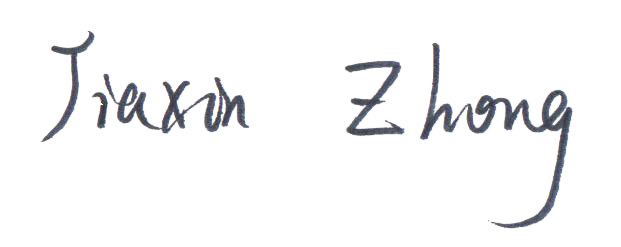
\includegraphics[scale=0.8]{img/Signature-EN1-20181030.png}
\vspace{-1em}

Dr. Jia-Xin Zhong

\newpage
\section{Comments from Editor}
\begin{commentbox}
    \lipsum[1]
\end{commentbox}

\subsubsection*{Responses}
\lipsum[2-3]

\subsubsection*{Changes}
\lipsum[3]


\newpage
\section{Comments from Reviewer 1}

\subsection{General comments}
\begin{commentbox}
    Here are the general comments from Reviewer 1.
\end{commentbox}



\subsubsection*{Responses}
Thank you for your comments and recommendation.
Reference~\cite{Zhong2022QuietZoneGeneration, Zhong2020InsertionLossThin}.
Figure~\ref{fig:ex} is an example image \cite{Zhong2020SphericalExpansionAudio}.

\begin{figure}[!htb]
    \centering
    \includegraphics[width = 0.4\textwidth]{example-image}
    \caption{Example image.}
    \label{fig:ex}
\end{figure}

\subsection{Major comment 1}
\begin{commentbox}
    \lipsum[3]
\end{commentbox}

\subsubsection*{Responses}
We added Sec.~IV.C entitled ``Computational efficiency'' in the revised manuscript to compare the calculation time of convolution models and the exact solution.
Equation~(\ref{eq:ex}) is the expression.

\begin{equation}
    f(x) = x^2 + 1.
    \label{eq:ex}
\end{equation}

\subsubsection*{Changes}
\begin{itemize}
    \item At line 405,
          Sec.~IV.C entitled ``Computational efficiency'' is added.
    \item Table~\ref{tab:2}.
\end{itemize}


\begin{table*}
    \caption{The position and weight coefficients for the uniform and optimal array configurations.}
    \label{tab:2}
    \centering
    \begin{tabular}{ccccc}
        \toprule
        \multirow{2}{4em}{Element index, $n$ }
          & \multicolumn{2}{c}{Position, $x_n$ (mm)}
          & \multicolumn{2}{c}{Weight coefficients, $w_n$}
        \\
          & Uniform array                                  & Optimal array
          & Uniform array                                  & Optimal array            \\
        \midrule
        1 & $-60$                                          & $-60$         & 1 & 1.99 \\
        2 & $-43$                                          & $-49$         & 1 & 1.17 \\
        3 & $-26$                                          & $-39$         & 1 & 1.15 \\
        4 & $-9$                                           & $-28$         & 1 & 0.92 \\
        5 & 9                                              & $-17$         & 1 & 0.62 \\
        6 & 26                                             & 40            & 1 & 1.19 \\
        7 & 43                                             & 50            & 1 & 1.73 \\
        8 & 60                                             & 60            & 1 & 1.51 \\
        \bottomrule
    \end{tabular}
\end{table*}

\subsection{Major comment 2}
\begin{commentbox}
    \lipsum[4]
\end{commentbox}

\subsubsection*{Responses}
Thank you for pointing out this typo.
We added $k_i$ in Eq.~(4) in the revised manuscript.

\subsubsection*{Changes}
Equation~(4)
\begin{equation}
    p_i(\bm\uprho_\mathrm{v}) =
    \frac{p_0}{2}
    \int_{-a}^a H_0(k_i\abs{\bm\uprho_\mathrm{v}-\bm\uprho_\mathrm{s}})
    u_i(\bm\uprho_\mathrm{s})
    \dd y_\mathrm{s}
    \tag{4}
\end{equation}
is revised as
\begin{equation}
    p_i(\bm\uprho_\mathrm{v}) =
    \frac{p_0}{2}
    \int_{-a}^a H_0(k_i\abs{\bm\uprho_\mathrm{v}-\bm\uprho_\mathrm{s}})
    u_i(\bm\uprho_\mathrm{s})
    \rev{k_i}
    \dd y_\mathrm{s}
    \tag{4}
\end{equation}


\subsection{Minor comments}
\begin{commentbox}
    \lipsum[5]
\end{commentbox}

\subsubsection*{Responses}
We have added descriptions for undefined symbols in the revised manuscript.

\subsubsection*{Changes}
\begin{itemize}
    \item
          Line 137, the descriptions
          ``\rev{$
                  \rho_\mathrm{s,<} = \min(\rho, \rho_\mathrm{s}),
                  \rho_\mathrm{s,>} = \max(\rho, \rho_\mathrm{s})
              $}''
          is added below Eq.~(8) in the revised manuscript.

    \item
          Line 160, the descriptions
          ``\rev{$
                  r_\mathrm{s,<} = \min(r,r_\mathrm{s}),
                  r_\mathrm{s,>} = \max(r,r_\mathrm{s})
              $}''
          is added below Eq.~(16) in the revised manuscript.
\end{itemize}



\newpage
\section{Comments from Reviewer 2}

\subsection{General Comments}
\begin{commentbox}
    \lipsum[6]

    \lipsum[7]
\end{commentbox}

\subsubsection*{Responses}
Thank you for the suggestion.

\subsubsection*{Changes}
\begin{itemize}
    \item Line 123, change 1.
    \item Line 234, change 2.
\end{itemize}


\newpage
\printbibliography
\addcontentsline{toc}{section}{References}


\end{document}
